\section{Mikrocontroller}
\label{Mikrocontroller}

%% Describes STM32F769I-DISCO, GPIO, registers, etc.
%% also some internal processing values
%% e.g. Taktrate am GPIO,
%%      Genauigkeit beim messen am GPIO
Die Spannungswerte lassen sich allerdings noch nicht messen oder darstellen.
Daher wird ein Bauteil benötigt, das die Spannungswerte digital darstellen kann.
Hierfür wird ein Mikrocontroller verwendet, der durch seine GPIO Pins und eingebauten ADC die Werte digital speichern kann.
Der STM32F769I-DISCO eignet sich, weil dieser zusätzlich ein integriertes 4 Zoll LCD Display
besitzt\cite{MikroControllerDatasheet_1}.
Durch die Bibliothek \textit{EmbSysLib} \cite{EmbSysLib}, wird die Software Implementierung des Displays zusätzlich
erleichtert. Zusätzlich wird das STM32F769-Disco Extension Board verwendet, um mehr
Anschluss-möglichkeiten am Mikrocontroller zu haben \cite{MikrocontrollerExtension}.
Im Folgenden werden die verwendeten Komponenten des Mikrocontrollers und wie die Messung und
Darstellung der Spannungswerte funktioniert, erläutert.

\subsection{GPIO}
Der STM32F769I-DISCO besitzt pro GPIO Pin vier 32-Bit Konfigurationsregister, zwei 32-Bit Datenregister
und ein 32-Bit Set-/Reset-Register \cite{MikroControllerDatasheet_1}.
Diese werden gebraucht um Daten zu lesen und zu senden.
\textit{General Purpose} bedeutet, dass die Pins für unterschiedlichste Zwecke für
Input/Output programmiert werden können \cite{RPI-GPIO}. \newline
Das Oszilloskop ist ein Messgerät, daher wird nur die Input Funktionalität des GPIO benötigt.
Um die analogen Spannungen messen und ausgeben zu können, müssen sie als digitaler Wert
im Mikrocontroller vorliegen. \newline
Die Umwandlung von analogem zu digitalem Wert übernimmt der ADC\cite{MikroControllerDatasheet_1}.
Deshalb muss unser Messeingang an einem GPIO Pin mit ADC Anschluss liegen, der \textit{ADC1} an GPIO Pin
\textit{PA4} eignet sich hierfür\cite{STM32F769_PinLayout, MikroControllerDatasheet_Pins}.
Am Extension Board liegt dieser Pin an Sensor Port \textit{S2-2} \cite{MikrocontrollerExtension}.


\subsection{ADC}

Der Mikrocontroller verwendet einen 12-Bit Analog-Digital-Converter (ADC).
Die analogen Werte werden also mit einer Auflösung von 12-Bit am \textit{PA4} gelesen und dann
in das 16-Bit Input-Data-Register (IDR) des Pins als digitaler Wert
geschrieben\cite{MikroControllerDatasheet_1}.
Deshalb kann der ADC zwischen $2^{12} = 4096$ verschiedene Spannungswerte im erlaubten Spannungsbereich,
$0V$ bis $3.3V$, am Pin messen\cite{MikroControllerDatasheet_1}.
Das Oszilloskop verwendet am Pin allerdings nur bis $3V$, dadurch ist das Teilungsverhältnis des Spannungsteilers
aus \ref{Spannungsteiler} einfacher zu berechnen. \newline
Hierbei sei gesagt, dass die Werte im IDR nicht direkt mit den gemessenen Spannungen korrellieren,
da der ADC einen Hex Wert zuweist, der im Bereich $0$ bis $4095$ liegt, dieser Wert aber nichts mit
dem Spannungswert zu tun hat. \newline
Ferner lässt sich die Grenze der Genauigkeit am ADC ausrechnen, also welcher Spannungsbereich denselben
Wert im IDR zugewiesen bekommt. \newline
Sei $\Delta U$ die Differenz zwischen zwei Spannungen, deren Hex-Werte im IDR sich um $1$
unterscheiden und $Hex = 4096$ die Anzahl der verschiedenen Werte im IDR,
dann
$$\Delta U = \frac{3.3V}{Hex} = 0.8mV$$
Das bedeutet, alle $0.8mV$ am Pin, verändert sich der IDR Wert. \newline
Folglich kann das Oszilloskop nicht genauer als auf $0.8mV$ messen.
\newline \newline
In \textit{EmbSysLib/Example/Src/Board/STM32F769-Discovery/config.h} wird nun ein
\texttt{Timer\_Mcu timer(Timer\_Mcu::TIM\_11, 100L)} Objekt erstellt\cite{EmbSysLib}. \newline
\texttt{100L} gibt an, dass alle $100\mu s$ ein Timer Interrupt ausgeführt werden soll.
Ein Timer Interrupt ruft dann die \texttt{virtual void TaskManager::Task::update()} Methode auf,
welche in einer abgeleiteten Klasse \texttt{MyTimer} überschrieben wurde,
der Code für das Oszilloskop ist nachzulesen in \cite{Oscilloscope_Code}.
Diese Methode liest einen Wert aus IDR, mittels der Methode \texttt{adc.get(adc\_A1)} des
globalen Objekts \texttt{adc} der Klasse \texttt{EmbSysLib::Hw::Adc\_Mcu},
und schreibt diesen in ein Array für die spätere Darstellung. \newline
Ein Wert wird alle $100\mu s$ gemessen, also
$$
\frac{1 \text{Wert}}{100 \mu s} \iff 10\frac{\text{Werte}}{ms}
\iff 10000 \frac{\text{Werte}}{s}
$$
Daraus folgt für die Frequenz $f$ der Messung
$$
f = 10000 \frac{1}{s} = 10 \si{\kilo\hertz}
$$

\subsection{Eingangsspannung berechnen}
Die Spannung am GPIO Pin \text{PA4} wird im Folgenden $U_{GPIO}$ genannt. \newline
Die Eingangsspannung wird als $U_{in}$ bezeichnet und die Spannung zwischen Opamp$_2$
und Spannungsteiler $(R_5, R_6)$ als $U_{vorST}$ angegeben.
\newline \newline
Die gemessene Spannung lässt sich wie folgt ausrechnen: \newline
Sei $U_{GPIO}$ die gemessene Spannung an \textit{PA4}, $Hex \in [0, 4095]$ der zugewiesene Wert im IDR
und $3V$ die maximale Spannung, die das Netzwerk aus \nameref{Schematic_all} an den \textit{PA4} gibt,
dann gilt
$$
	U_{GPIO} = \frac{Hex \cdot 3V}{4095}
$$
ist die Spannung an \textit{PA4} in Volt.
\newline \newline
Die Spannung $U_{GPIO}$ ist allerdings nicht die Eingangsspannung am Oszilloskop, die tatsächlich gemessen werden soll, da
das Opamp-Netzwerk aus \ref{Eingangsspannung bereinigen} diese, für den GPIO Pin, bereinigt.
Es gilt nun, diese Bereinigung Schritt für Schritt in der Software wieder zurückzurechnen, um die Eingangsspannung zu erhalten. \newline
Der Spannungsteiler aus \ref{Spannungsteiler} teilt $U_{vorST}$
zu $U_{GPIO}$, also gilt laut Spannungsteilerregel
$$
	U_{GPIO} = \frac{U_{vorST} \cdot 100 \Omega}{333 \Omega + 100 \Omega}
$$
Daraus folgt
$$
	U_{vorST} = \frac{U_{GPIO} \cdot (333 \Omega + 100 \Omega)}{100 \Omega}
$$
\newline\newline
Um dann die Eingangsspannung zu erhalten, muss man lediglich die Offset Spannung $U_{offset}$
von $U_{vorST}$ subtrahieren, es folgt
$$
	U_{in} = U_{vorST} - U_{offset}
$$
wobei $U_{in}$ die Eingangsspannung, die gemessen werden soll, darstellt.


\subsection{Display}

Das Display ist ein $4$-Zoll LCD-TFT-Display mit einer Auflösung von \newline $800 \times 472 \si{px}$
und einer Bildwiederholrate von 30\si{\hertz} \cite{MikroControllerDatasheet_1}.
Da für die Frequenz der Messung $10 \si{\kilo\hertz} > 30 \si{\hertz}$ gilt,
misst der Mikrocontroller deutlich schneller, als er die Messwerte darstellen könnte.
Die gemessenen Werte müssen dementsprechend zumindest temporär, bis zur Darstellung auf dem Display,
in einer Datenstruktur, z.B. einem Array, zwischengespeichert werden, siehe \cite{Oscilloscope_Code}.
Sobald das Array gefüllt wurde, wird es ausgegeben.
Auf dem gesamten Display werden also ca. 800 gemessene Werte, ein Wert pro Pixel auf der Zeitachse,
dargestellt. \newline
In der Zeit vom gefüllten Array bis zur
vollständigen Ausgabe ZEIT MESSEN UND HIERREIN SCHREIBEN wird das Array weder geleert noch überschrieben,
da sonst die alten Daten, die eventuell noch nicht ausgegeben wurden, verloren gehen.
Daher wird beim Oszilloskop der Fokus auf korrekt gemessene, aufeinanderfolgende Werte in einer
Stichprobe anstatt auf eine kontinuierliche Messung gelegt.
\newline \newline
Für die Darstellung wird ein Koordinatensystem mit zwei Achsen, Zeit- und Spannungsachse,
auf dem Display aufgemalt.
Die Spannungsachse zeigt die Werte $-15V$ bis $+15V$, in $1V$ Schritten.
Die Zeitachse zeigt die Zeiten von $0s$ bis $0.1s$, in Schritten von $0.01s$.
Die jeweiligen Werte müssen nun einem x- und y-Wert auf dem Display zugeordnet werden,
um dort einen Pixel zu malen. Dieser Pixel soll den gemessenen Wert darstellen. \newline
Hierfür werden zwei Konstanten für die Skalierung auf den Achsen definiert,
\texttt{pixelPerVolt} und \texttt{pixelPerSecond}.
Diese werden benötigt um den jeweiligen Spannungs- und Zeitwert, z.B eine Spannung im Bereich
$[1,2]V$ auch auf dem Display zwischen den Pixeln für $1V$ und $2V$ anzuzeigen.
Die Konstante \texttt{pixelPerVolt} gibt an, wieviele Pixel in einem $1V$ Intervall auf der
y-Achse auf dem Display liegen.
Die andere Konstante \texttt{pixelPerSecond} gibt an, wieviele Pixel in einem $0.01s$ Intervall
auf der x-Achse liegen. \newline
Mit diesen beiden Konstanten und den gemessenen Werten, lassen sich die Koordinaten des zu setzenden
Pixels errechnen, durch
$$
\texttt{y}(\texttt{volt}) = \begin{cases}
	\texttt{ymax}/2 - \texttt{volt} * \texttt{pixelPerVolt} & \texttt{volt} \ge 0 \\
	\texttt{ymax}/2 + \texttt{volt} * \texttt{pixelPerVolt} & \text{sonst} \\
\end{cases}
$$
Die positiven Spannungswerte befinden sich in der oberen Hälfte des Displays, also $\le \texttt{ymax}/2$,
die negativen Werte liegen in der unteren Hälfte. \newline
Die Zeitwerte werden einfach von der ersten x-Koordinate, also $0s$ startend, pro Spannungswert inkrementiert.
Da es genau soviele gemessenen Werte wie Pixel zwischen der ersten x-Koordinate bei $0s$
und der letzten bei $0.1s$ gibt, und konstant gemessen wird, ist die Zeiteinteilung trivial. \newline
Eine einfache Messung sieht so aus:
\begin{figure}[h]
	\centering
	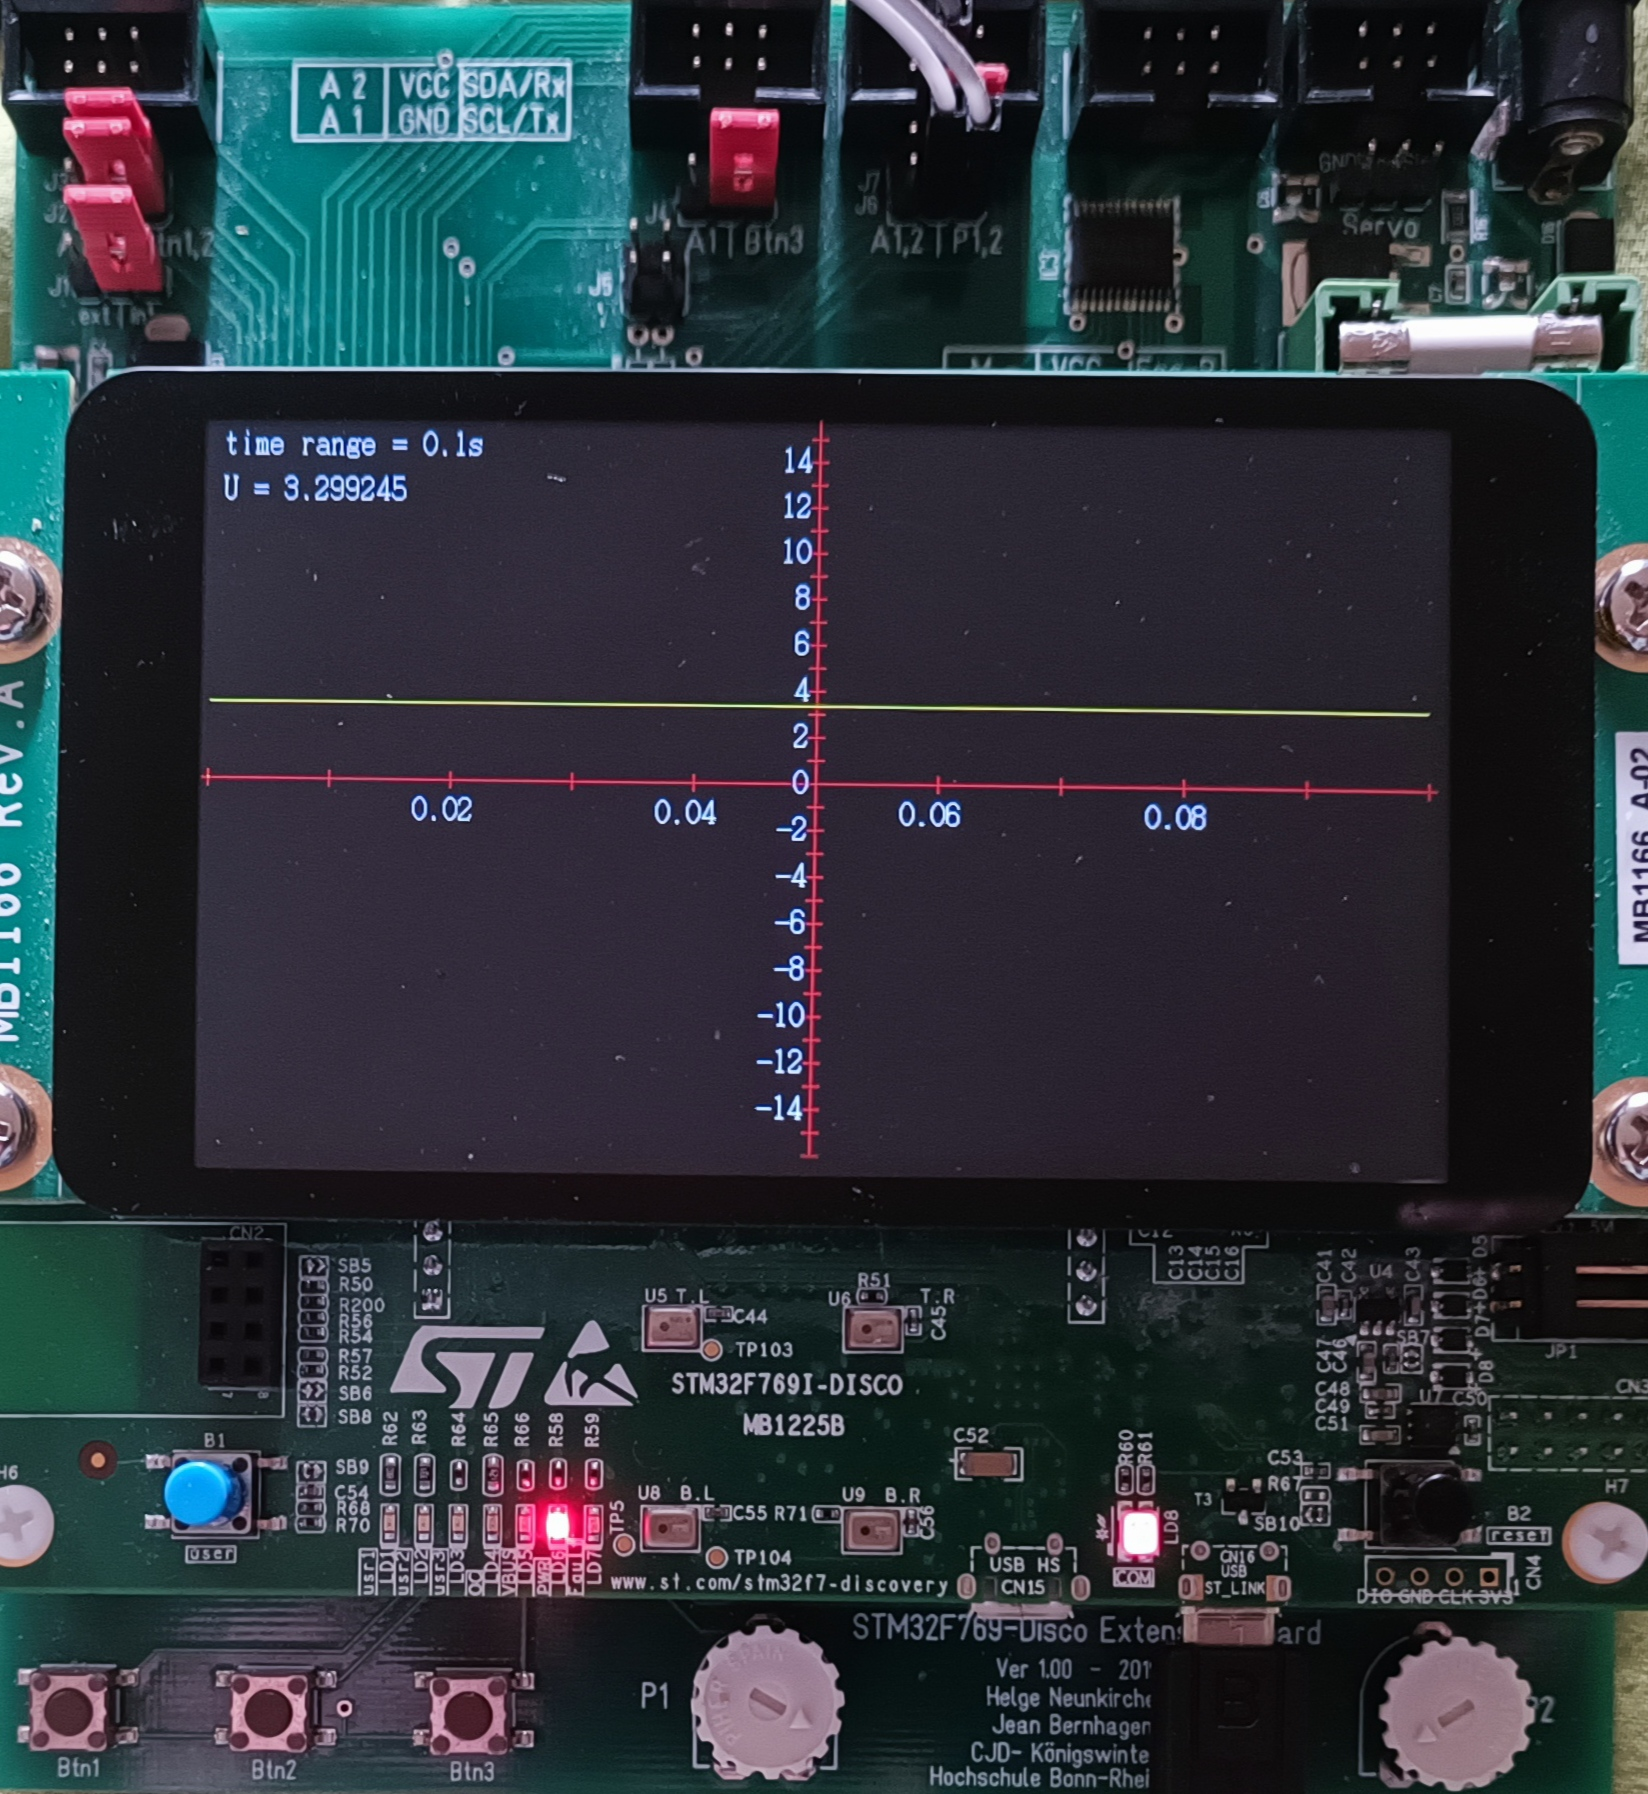
\includegraphics[scale=0.125]{images/messung3.3V.jpg}
	\caption{Messung von konstanten $3.3V$ durch das Oszilloskop}
\end{figure}
\newline
Wenn eine Messung vollständig dargestellt wurde, kann durch betätigen von \textit{Btn3},
auf dem Extension Board, eine neue Messung gestartet werden.
